\section{The experiment}
The main question we would like to answer in the experiment is: \textit{Would the introduction of generated spelling errors allow a chatbot to perform better in a Turing Test?} Given the discussed literature, our hypothesis is that generated spelling errors would indeed allow a chatbot to perform better in a Turing Test. The experiment will now be described in detail.


\subsection{Participants}
The participants were 20 students of Utrecht University who volunteered to take part in the experiment. Participants ranged in age from 18 to 26, with a mean age of 21.65. Of the participants, exactly 50\% were male and 50\% female. The largest group (40\%) had not previously heard of the Turing Test, the minority (25\%) had prior knowledge of it and the rest (35\%) had heard of the test but not in detail.


\subsection{Procedure}
The participants were placed in front of a computer with two chat windows open on Skype, simultaneously with \textit{Person 1} and with \textit{Person 2}. The participants were then told that they had to converse by chat interface with two people and they had to choose which one of the persons was a real person and which one was a computer. There was a time limit set at three minutes, but they could stop at any moment before, once they thought they knew who the computer was. They were prohibited from using emoticons and they could only ask one question at a time. Each of the participants did two rounds of conversations in total. The participants were explicitly told that the second round was a new conversation so they won't necessarily be influenced by their first conversation. During the entire experiment, Person 1 was the chatbot while Person 2 was the same real person. We chose to use the same human participant during the entire experiment to have a constant bias rather than a variable bias.

Behind the scenes, we conducted this experiment in a Wizard of Oz set-up, in which the answers given by the chatbot were copied by a human controller verbatim to act as Person 2's answers in the Skype interface; the participant's questions were copied verbatim as well and fed to the chatbot. The human controlling the chatbot followed a schedule, see Table~\ref{schedule}, so that the first ten participants talked to the chatbot Mike\footnote{http://www.eslfast.com/robot/english\_tutor.html} and the last ten participants talked to the chatbot Rose\footnote{http://brilligunderstanding.com/rosedemo.html} during both rounds.

\begin{table}[!ht]
   \begin{center}
      \caption{Distribution of conversations}
      \label{tabdistributionofconversations}
      \vskip 0.12in
      \begin{tabular}[center]{| c | c | c |}
         \hline
         Chatbot & Control & With spelling errors \\
         \hline \hline
         Rose & 10 & 10\\
         Mike & 10 & 10\\
         \hline
      \end{tabular}
   \end{center}
\end{table}

The chatbots Mike and Rose have both been chosen due to their performance in the Loebner Prize\footnote{http://www.loebner.net/Prizef/loebner-prize.html} in the last two years. Mike is a language chatbot that aims at helping users with their English skills; it is also equipped to answer a wide scope of questions, ranging from geography and politics, to irregular verbs. Rose, on the other hand, was declared the most human-like chatbot in the latest Loebner Prize Competition. It is a self-described \textit{computer-nerd} and has its own personality, in a way. Rose is based on the ChatScript engine\footnote{http://brilligunderstanding.com/technology.html footnote} which is equipped with a powerful pattern matching mechanism aimed at detecting meaning; the engine also remembers user interactions across conversations.

The schedule indicated that each person had one conversation with the chatbot without added spelling errors (the control group) and the other conversation with the same chatbot with the introduction of spelling errors. Half of the participants were in the control group in the first conversation; while the other half were in the control group in the second conversation. We used a script to generate spelling errors based on the most common misspellings in English made by humans(citation needed). The spelling errors were introduced according to the length of the sentence and a chance variable. The maximum amount of errors is calculated as 10\% of the amount of words in the sentence rounded down. And then there is a chance of 1/3 to introduce a spell error. The algorithm checks the words in the sentence given by the chatbot against a library of the most commonly misspelled words. When a match is found it replaces the original word with the misspelled word in the sentence.

A questionnaire was used to gather data on the experiment. First, the participants were asked basic questions about the gender and age of the participant and their participant number. The participant number is needed as a reference to the participant. The age and gender are needed for further data analysis.

After each of the two rounds of conversations, the participants proceeded to fill in questions regarding the conversations they just had. The questions for the first and second conversation are identical. First they are asked which person they think was the machine. This is answered with a slider from 0 to 100, where 0 means \textit{Person 1 is definitely the computer} and 100 means \textit{Person 2 is definitely the computer} and 50 means \textit{I have no idea who the computer is.} This number is then processed in the data analysis. Secondly, they need to give a reason as to why they gave the answer to the previous question. This gives us some insight into the thinking and decision making of the participants. Finally, the time duration of the experiment is filled in. Since participants are allowed to stop before the time limit, we need to know if they did so. After filling in these questions for the first round of conversations, the participants continued with the second round of conversations.

After participating in both rounds of conversations and answering questions regarding those conversations, the participants are asked about their knowledge of the Turing Test. This question is needed to find any correlation between prior knowledge of the test and how well they do. The question is asked last to limit any influence of the questionnaire on the experiment. Finally there was room for additional remarks.


\subsection{Results}
Our experiment was conducted using a within-subjects design. We tested the effect of a repeated measures procedure, where the participants are used both in the control group and the experiment group. As previously mentioned, by asking participants to provide probabilistic answers, we were able to compare the differences in the measured dependant variable between different conditions, namely with the introduction of spelling errors and without. To test our main hypothesis, namely that the introduction of generated spelling errors would allow a chatbot to perform better in a Turing test, a Wilcoxon signed-rank test has been performed, yet the result was not statistically significant (Z = -1.14, p $<$ 0.05).

\begin{figure}[ht]
   \begin{center}
      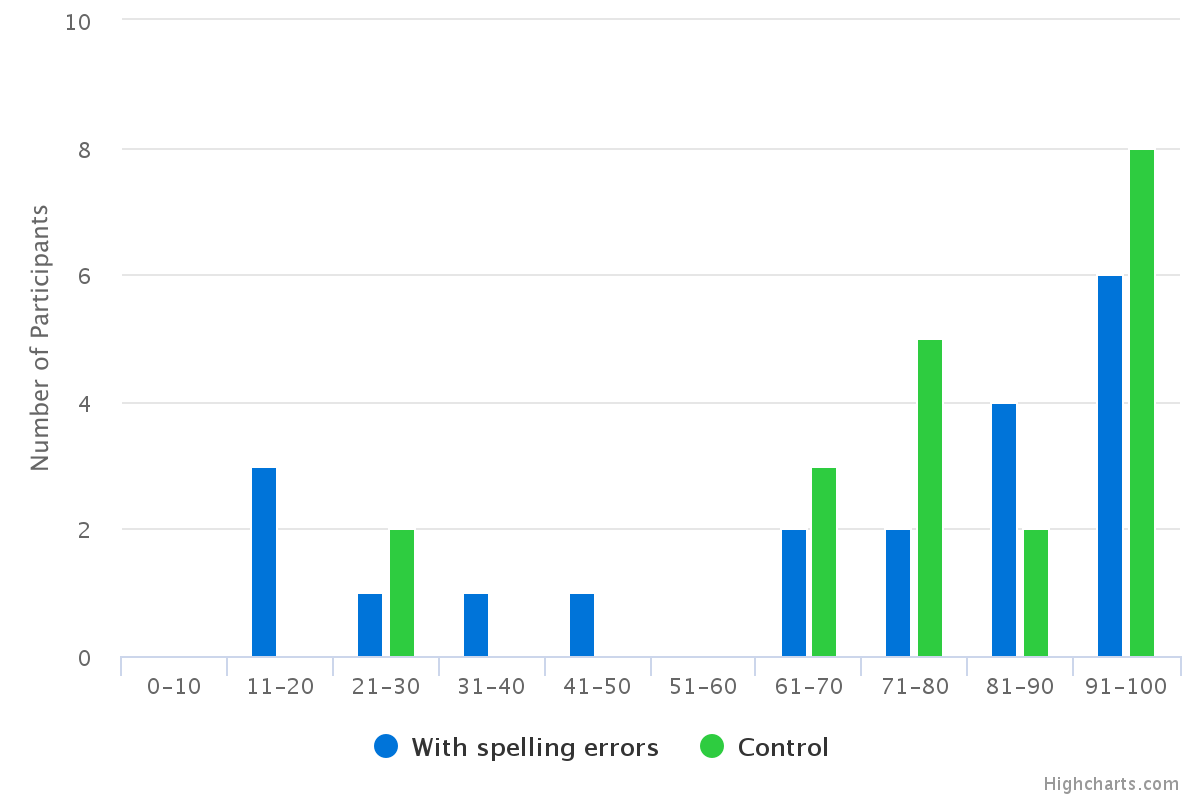
\includegraphics[width=\columnwidth]{chart}
   \end{center}
   \caption{Results of the turing test.\\ Where 0-100 is the percentage of certainty whether Person 2 was indeed a computer}
   \label{chart}
\end{figure}

From an analysis of the post-experiment questionnaire we learn that 40\% of participants have never heard of the Turing Test. 35\% of participants had a vague notion of what the test is and 25\% of participants knew exactly what the Turing Test is.

It is worth noting that we have found a significant positive correlation between prior knowledge of the Turing Test and the correct identification of the computer as the computer (r(40) = .39, p $<$ 0.05). Further, no significant correlation has been found between the amount of time it took participants to confidently determine the identity of the computer, and the correct identification of the computer as the computer.

Figure~\ref{chart} allows us to explore the distribution of the participants responses, both with and without the introduction of spelling errors. Although a statistically significant difference was not found, the two distributions are visually different, with and without the introduction of spelling errors. When spelling errors were introduced, 30\% of participants indicated that they are more confident about the chatbot not being the computer, compared to 10\% when errors were not introduced. Furthermore, when spelling errors were introduced, we find that 30\% of participants indicated the highest level of confidence in the chatbot being the computer, compared to 40\% when spelling errors were not introduced. This might show that, on average, the participants were less certain of the chatbot's true identity when spelling errors were introduced.
